\section{Discussion} \label{sec:discussion}
In this section, we report qualitative analysis of user-aspect reliabilities \{$r_n$\} and word embeddings \{$v_w$\} learned by our proposed CrowdQM model. For brevity, we focus our analysis on our largest subreddit, askscience.

\subsection{Aspect Reliability Analysis}
We evaluate learned user reliabilities through users commenting on a post with a \emph{submission flair}. A submission flair is manually curated and denotes post's category, and this information is not used in our model. Specifically, for each post $m$, we compute the \emph{user-post reliability} score, $R_{m,n}$, for every user $n$ who commented on the post. We then ranked these scores for each category and report top-10 \emph{author flairs} for few categories in Table \ref{tab:modelAlignment2}.

\begin{spacing}{1}
\begin{longtable}{l}
\caption[Author flairs per post categories]{Most reliable author flairs with their corresponding post categories according to user-post reliability score, $R_{m, n}$.
} \\
\hline  \toprule
\endfirsthead

\hline
{\bfseries \tablename\ \thetable{} -- continued from previous page} \\ \hline
\endhead

\hline %{\bfseries \tablename\ \thetable{} Continued on next page} \\\hline
\endfoot

%\hline
\endlastfoot
 \multicolumn{1}{c}{Post Category: Computing} \\ \hline
Embedded Systems, Software Engineering , Robotics \\
Computer Science \\
Quantum Optics, Singular Optics \\
Robotics, Machine Learning, Computer Vision, Manipulators \\
Computer Science \\
High Performance Computing, Network Modeling and Simulation \\
Biomechanical Engineering, Biomaterials \\
Machine Learning, Deep Architectures, Scientific Computing  \\
Machine Learning, Deep Architectures, Scientific Computing\\
Programming Languages, Computer Security \\
\hline

\multicolumn{1}{c}{Post Category: Archaeology} \\ \hline
Archaeology, Maya Stone Tools, Geoscience \\
Global Health, Tropical Medicine \\
Control, Robotics Engineering, Industrial Robotics \\
Archaeology, Collapse of Complex Societies \\
Archaeology, Archaeometallurgy \\
Criminal Justice  \\
Computational and Evolutionary Archaeology \\
Evolutionary Biology, Plant-Herbivore Systems \\
Computational and Evolutionary Archaeology \\
Archaeology, Collapse of Complex Societies \\
\hline

\multicolumn{1}{c}{Post Category: Biology} \\ \hline
Animal Cognition  \\
Cell and Developmental Biology  \\
Biochemistry, Molecular Biology, Enzymology  \\
Genetics, Cell biology, Bioengineering \\
Computational Physics, Biological Physics \\
Aquatic Ecology and Evolution, Active Acoustics \\
Genomic Instability, Cancer Development \\
Biochemistry, Genomics, Proteomics, Mass Spectrometry \\
Neuroscience, Psychopharmacology \\
Genetics and Genomic Sciences \\
\hline
\multicolumn{1}{c}{{Post Category:Linguistics}} \\ \hline
Linguistics, Hispanic Sociolinguistics  \\
Comparative Political Behaviour \\
Historical Linguistics, Language Documentation \\
Linguistics, Hispanic Sociolinguistics \\
Historical Linguistics, Language Documentation  \\
Cognitive Modeling \\
Nanostructured Materials, Heterogeneous Catalysis \\
Auditory Science  \\
Cognitive Modeling \\
Linguistics, Phonetics and Phonology, Sound Change \\
\hline

\multicolumn{1}{c}{{Post Category: Medicine}} \\ \hline
Infectious Diseases, Pulmonary Immunology \\
Biomedical Engineeering, Biomechanics, Biomaterials \\
Pediatric Neurology \\
Anesthesiology, Post-Operative Pain, Traumatic Brain Injuries \\
Molecular Biology, Musculoskeletal Research \\
Immunology, Immune Regulation, Infectious Diseases  \\
Molecular Biochemistry, DNA Damage Repair \\
Virology, Molecular Biology, Orthopoxviruses \\
Veterinary Medicine, Canine Lymphoma \\
Bioengineering, Cardiovascular Imaging  \\
\hline

\multicolumn{1}{c}{{Post Category: Psychology}} \\ \hline
Clinical Psychology, Psychotherapy, Behavior Analysis  \\
International Relations, Comparative Politics  \\
Neuropsychology \\
Psychology, PTSD, Trauma, and Resilience  \\
Cognitive Neuroscience, Neuroimaging, fMRI  \\
Psychology, Legal psychology, Eyewitness testimonies   \\
Experimental Psychology, Social Cognition and Statistics  \\
Clinical Psychology   \\
Clinical Psychology, Sleep, Insomnia \\
Visual Cognition, Cognitive Neuroscience  \\
\bottomrule
%\end{tabular}
\label{tab:modelAlignment2}
\end{longtable}
\end{spacing}

The top-performing \emph{author flairs} for each category are experts for that domain.
For instance, for the Computing category highly reliable users have author flairs like Software Engineering and Machine Learning, while for Linguistics authors with flairs Hispanic Sociolinguistics and Language Documentation rank high. These results align with our hypothesis that in-domain experts should have higher reliabilities.
We also observe that few out of domain authors being ranked high, such as, authors with flairs like Comparative Political Behavior and Nanostructured Materials in the Linguistic category. This diversity could be due to the interdisciplinary nature of that domain.
Our model, thus, can be used by the moderators of the discussion forum to identify and recommend potential reliable users to respond to new submission posts of a particular category.

\begin{figure}[h]
%\vspace{-0.1in}
  \begin{subfigure}{0.5\textwidth}
  \centering
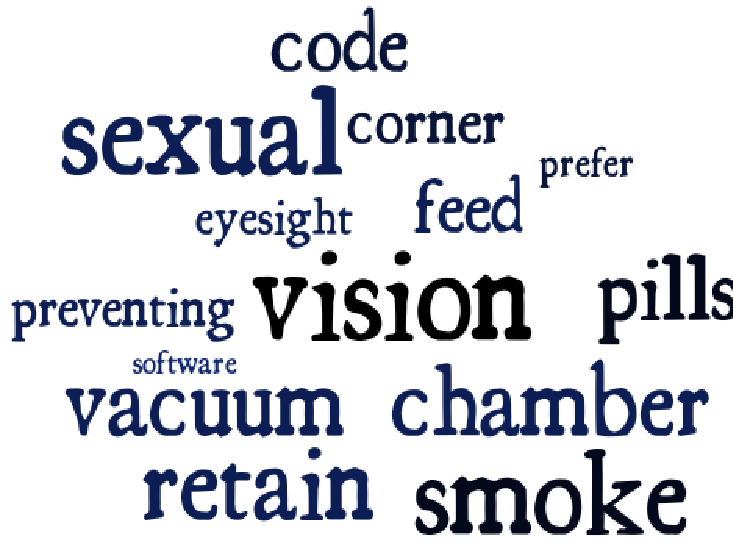
\includegraphics[scale=0.5]{images/Health.pdf}
\caption{Health}
\end{subfigure}
  \begin{subfigure}{0.5\textwidth}
  \centering
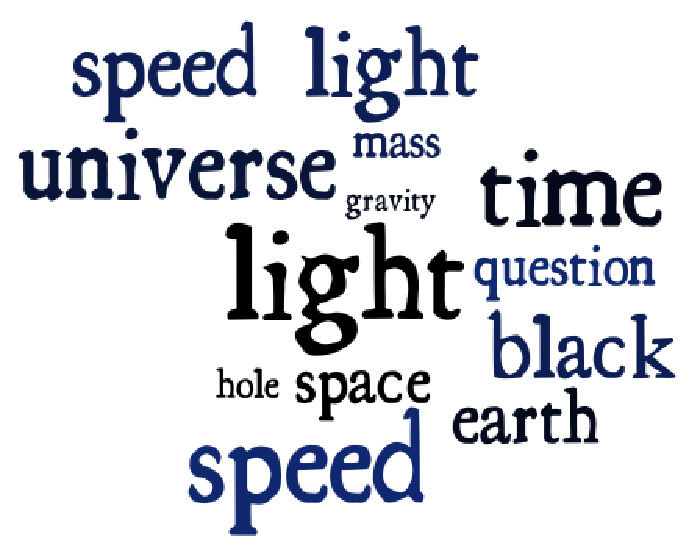
\includegraphics[scale=0.5]{images/Cosmos.pdf}
\caption{Cosmos}
\end{subfigure}
  \begin{subfigure}{0.5\textwidth}
  \centering
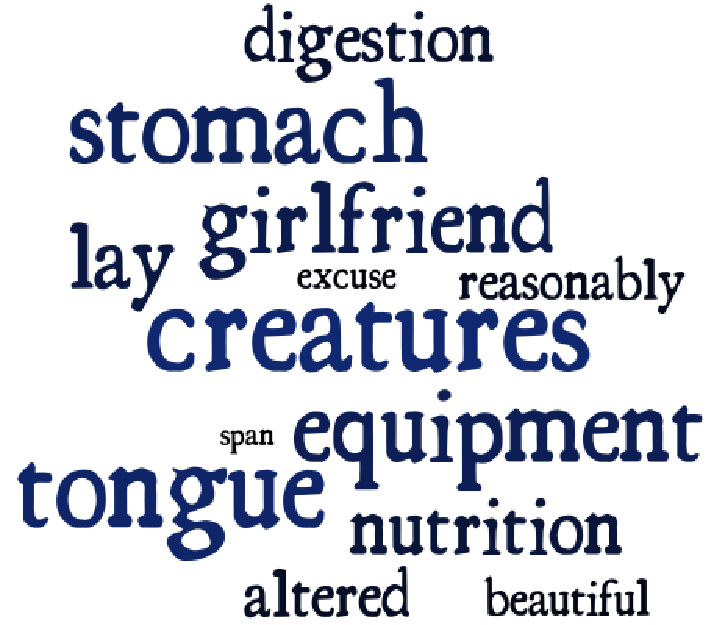
\includegraphics[scale=0.5]{images/Diabetes.pdf}
\caption{Diabetes}
\end{subfigure}
  \begin{subfigure}{0.5\textwidth}
  \centering
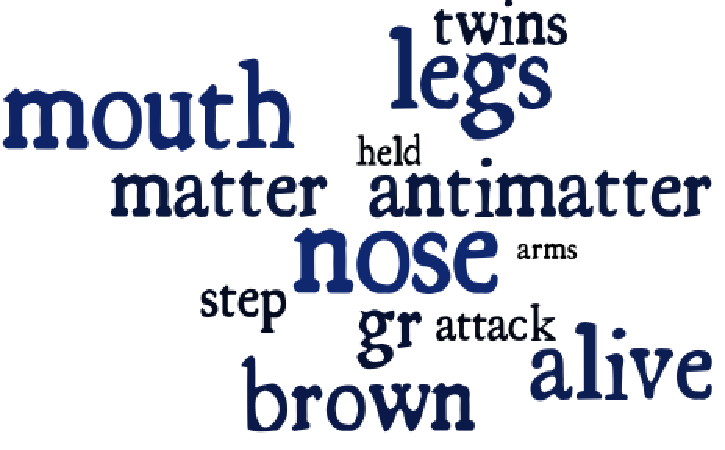
\includegraphics[scale=0.56]{images/Oceanography.pdf}
\caption{Oceanography}
\end{subfigure}
\caption{Top words for highly correlated aspects between user reliability and user karma.}
\label{fig:modelTopics}
\end{figure}

To further analyze the user reliability, we qualitatively examine the aspects with the largest reliability value of highly upvoted users in a post category. First, we identify users deemed reliable by the community for a category through a \emph{karma} score. Category-specific user \textit{karma} is given by the average upvotes the user's comments have received in the category.  We then correlate the category-specific user \textit{karma} with her reliability score in each $k \in K$ aspect, $\bm{r}_n^{(k)}$ to identify aspects relevant for that category.
Figure \ref{fig:modelTopics} shows the top words of the highest correlated aspects for some categories. The identified words are topically relevant thus our model associates aspect level user reliability coherently.
Interestingly, the aspects themselves tend to encompass several themes, for example, in the Health category, the themes are software and health. Or in the Oceanography category, the themes are around animal's physiology and matter.

\subsection{Word Embedding Analysis}

\begin{table}[tbh]
 %\captionsetup{font=small}
 \centering
 %\small
\resizebox{0.97\linewidth}{!}{
\begin{tabular}{ c | c | c | c | c | c }
\toprule
\multicolumn{2}{c| }{{Liquid}} &  \multicolumn{2}{c|}{{Cancer}} & \multicolumn{2}{c}{{Quantum}} \\ \hline
word2vec         & CrowdQM   & word2vec   & CrowdQM  & word2vec             & CrowdQM      \\ \hline
unimaginably     & gas       & mg         & disease  & search results       & model        \\
bigger so        & chemical  & curie      & white    & sis                  & energy       \\
two lenses       & solid     & wobbly     & cell     & shallower water      & particle     \\
orbiting around  & air       & subject    & food     & starts rolling       & mechanics  \\
fire itself      & material  & "yes" then & complete & antimatter galaxies  & mathematical \\
\bottomrule
\end{tabular}}\vspace{8mm}
\resizebox{0.6\linewidth}{!}{
\begin{tabular}{ c | c | c | c }
\toprule
\multicolumn{2}{c|}{{Life}} & \multicolumn{2}{c}{{Planet}} \\ \hline
word2vec      & CrowdQM    & word2vec       & CrowdQM \\ \hline
molaison      & species    & esther         & earth \\
around        & natural    & missing leg    & star \\
machos        & nature     & chimps         & plane \\
brain         & production & while drinking & land\\
"dark" matter & size       & living off     & building \\
\bottomrule
\end{tabular}
}
\caption{Similar words identified using embeddings learned by CrowdQM, and initial word2vec, for the askscience subreddit. The left and right columns correspond to word2vec and CrowdQM models respectively.}
\label{tab:WordSym}
\end{table}


The CrowdQM model updates word embeddings to better model semantic meaning of the comments. To evaluate the embeddings, we first identify the most representative aspect for each category. We denote the highest weighted aspect from the mean aspect distribution \{$\bm{p}_m$\} of all posts belonging to a category as the most representative aspect of that category.
Then, we extract frequent terms of that aspect and find its most similar keywords using cosine distance between the learned word embeddings.

The left column for each term in Table \ref{tab:WordSym} are the most similar terms returned by the initial embeddings from word2vec model while the right column reports the results from updated embeddings \{$\bm{v}_\omega$\} from our CrowdQM model.
We observe that there is a lot of noise in words returned by word2vec model as they are just co-occurrence based while words returned by our model are semantically similar and describe similar concepts. This improvement is because our model updates word embeddings in a trust aware manner such that they are similar to terms used by responses from reliable users.
